% Beamer slide deck for Mathematical Physics
% "Mathematical Physics"
% Chapter 5: Bessel Functions
% Original-based second trimming pass; supplied style retained.

\documentclass[11pt]{beamer}

\usepackage[utf8]{inputenc}
\usepackage[T1]{fontenc}
\usepackage{lmodern}
\usepackage{amsmath,amssymb}
\usepackage{graphicx}

\usetheme{Madrid}

\author[]{Compiled by Jake W. Liu}
\title[Bessel Functions]{Chapter 5: Bessel Functions}
\subtitle{Mathematical Physics}
\date{\today}

\setbeamertemplate{navigation symbols}{}
\setbeamertemplate{frametitle continuation}[from second]

% Per-section TOC frames removed to keep the deck within 60 slides.

\usepackage{Kyushu}

% Neutralize \index so source markup (if any) is harmless.
\makeatletter
\@ifundefined{index}{\newcommand{\index}[1]{}}{\renewcommand{\index}[1]{}}
\makeatother

\begin{document}

\newcounter{sfchapter}
\setcounter{sfchapter}{5}
\renewcommand{\thesection}{\arabic{sfchapter}.\arabic{section}}
\numberwithin{equation}{section}

\begin{frame}[c]\titlepage
\end{frame}

\begin{frame}{Outline}
\tableofcontents
\end{frame}

\begin{frame}[allowframebreaks=1.00]{Where we are going}
\footnotesize
\textbf{Why Bessel functions?} A drumhead, a circular waveguide, or sound in a pipe all obey the
Helmholtz equation \((\nabla^2+k^2)u=0\). In polar coordinates
\(\nabla^2u=u_{rr}+\frac1ru_r+\frac1{r^2}u_{\theta\theta}\). Look for a single angular mode
\(u=R(r)\,e^{im\theta}\):
\begin{itemize}
  \item \(u_{rr}=R''e^{im\theta}\), \(\;u_r=R'e^{im\theta}\), \(\;u_{\theta\theta}=(im)^2Re^{im\theta}=-m^2Re^{im\theta}\);
  \item substitute and cancel the common factor \(e^{im\theta}\):
        \(R''+\frac1rR'-\frac{m^2}{r^2}R+k^2R=0\);
  \item multiply by \(r^2\): \(r^2R''+rR'+(k^2r^2-m^2)R=0\).
\end{itemize}
With \(x=kr\) and \(y(x)=R(r)\) (as in Chapter~3) this is Bessel's equation of integer order \(m\):
\begin{equation}
  x^2 y''(x)+x y'(x)+(x^2-m^2)y(x)=0.
  \label{eq:bessel-ode-opening}
\end{equation}
\par\framebreak\par
\textbf{This chapter develops}
\begin{itemize}
  \item a generating function for the whole family \(J_m\), and from it the power series;
  \item recurrences linking neighbouring orders and derivatives;
  \item a real integral representation;
  \item the behaviour for small and for large \(x\);
  \item the second solution \(Y_m\), the Hankel functions \(H^{(1)},H^{(2)}\) (traveling waves), and the
        Fourier--Bessel series on the disk;
  \item half-integer orders, where everything reduces to elementary functions: the spherical Bessel
        and Hankel functions.
\end{itemize}
Throughout, \(m,n\) are integers unless stated otherwise; in small- and large-\(x\) limits the order is held
fixed.
\end{frame}

% ======================================================================
\section{Generating function}
% ======================================================================

\begin{frame}[allowframebreaks=1.00]{Generating function for the family $\{J_m\}$}
\footnotesize
\textbf{The idea.} Find one simple function whose Fourier coefficients are all the \(J_m\) at once.
Physics suggests a candidate: a plane wave.

\textbf{Step 1: a plane wave is a solution.} \(u=e^{iky}\) solves \((\nabla^2+k^2)u=0\) (since
\(\partial_y^2e^{iky}=-k^2e^{iky}\)). In polar coordinates \(y=r\sin\theta\), so with \(x=kr\) it reads
\[
 u=e^{ix\sin\theta}.
\]
\textbf{Step 2: expand it in angular modes.} It is \(2\pi\)-periodic in \(\theta\), so it has a Fourier series
\(e^{ix\sin\theta}=\sum_mc_m(x)\,e^{im\theta}\). Each term \(c_m(x)e^{im\theta}\) is itself a solution (the Laplacian
does not mix different \(e^{im\theta}\)), and it is finite at \(r=0\). So by the opening slide \(c_m\) solves
Bessel's equation and is regular at \(0\): we expect \(c_m=J_m\).
\par\framebreak\par
\textbf{Step 3: rewrite with \(t=e^{i\theta}\).} Then \(e^{im\theta}=t^m\), and
\(\sin\theta=\frac{e^{i\theta}-e^{-i\theta}}{2i}=\frac{t-t^{-1}}{2i}\), so
\[
 ix\sin\theta=ix\cdot\frac{t-t^{-1}}{2i}=\frac x2\bigl(t-t^{-1}\bigr).
\]
\textbf{Definition.} We therefore \emph{define} \(J_m(x)\) as the coefficients of the Laurent series
\begin{equation}
 g(x,t)=\exp\left[\frac x2(t-t^{-1})\right]
       =\sum_{m=-\infty}^{\infty}J_m(x)t^m,\qquad t\ne0,
 \label{eq:genf}
\end{equation}
and check on the next frame that these \(J_m\) are the Chapter~3 series. Notation: \([t^m]g\) means ``the
coefficient of \(t^m\) in \(g\)'', so \(J_m(x)=[t^m]g(x,t)\).

\textbf{What \(g\) is good for.} Multiplying out \(g\) gives the power series of every \(J_m\); differentiating
\(g\) gives relations between neighbouring orders.
\end{frame}



\begin{frame}[allowframebreaks=1.00]{Reading off the integer-order series}
\footnotesize
\textbf{Goal.} The generating function \eqref{eq:genf} defines $J_m(x)$ as a coefficient. We
want the explicit power series of that coefficient, to compare with Chapter~3.

\textbf{Step 1: expand each exponential.} Split \(g=e^{xt/2}\cdot e^{-x/(2t)}\) and use
\(e^u=\sum_ju^j/j!\), with \(u=xt/2\) in the first factor and \(u=-x/(2t)\) in the second:
\[
 e^{xt/2}=\sum_{j=0}^{\infty}\frac{(x/2)^j}{j!}t^j,
 \qquad
 e^{-x/(2t)}=\sum_{k=0}^{\infty}\frac{(-1)^k(x/2)^k}{k!}t^{-k}.
\]
\textbf{Step 2: multiply.} Multiplying a term of the first series by a term of the second,
\[
 g(x,t)=\sum_{j,k\ge0}\frac{(-1)^k}{j!\,k!}
                  \left(\frac x2\right)^{j+k}t^{j-k}.
\]
(Both series converge absolutely for \(t\ne0\), so the terms may be grouped in any order.)

\textbf{Step 3: collect one power of \(t\).} The power of \(t\) is \(j-k\). To get \(t^m\) (with \(m\ge0\)) we
need \(j-k=m\), that is, \(j=k+m\). Then \(j!=(k+m)!\) and \(j+k=2k+m\). Summing over the remaining
index \(k\):
\begin{equation}
 J_m(x)=[t^m]g(x,t)=\sum_{k=0}^{\infty}
 \frac{(-1)^k}{k!(m+k)!}\left(\frac x2\right)^{2k+m},
 \qquad m=0,1,2,\ldots.
 \label{eq:series}
\end{equation}
\par\framebreak\par
For example,
\begin{align*}
 J_0(x)&=1-\frac{x^2}{4}+\frac{x^4}{64}-\frac{x^6}{2304}+\cdots,\\
 J_1(x)&=\frac x2-\frac{x^3}{16}+\frac{x^5}{384}+\cdots,\\
 J_2(x)&=\frac{x^2}{8}-\frac{x^4}{96}+\frac{x^6}{3072}+\cdots.
\end{align*}
These are the series obtained from the differential equation in Chapter~3, so the
plane-wave guess was right: a single generating function holds all integer orders at once.
\end{frame}

\begin{frame}[allowframebreaks=1.00]{General order series}
\footnotesize
\textbf{Why general order?} Wedge-shaped regions and the spherical problems at the end of this chapter
lead to Bessel's equation with a noninteger order $\nu$ in place of $m$. Chapter~3's
Frobenius solution with root $r=\nu$ is the same series with $(k+m)!$ replaced by
$\Gamma(k+\nu+1)=(\nu+k)(\nu+k-1)\cdots(\nu+1)\Gamma(\nu+1)$:
\begin{equation}
 J_\nu(x)=\sum_{k=0}^{\infty}
 \frac{(-1)^k}{k!\,\Gamma(k+\nu+1)}
 \left(\frac x2\right)^{2k+\nu},\qquad x>0.
 \label{eq:series-gamma}
\end{equation}
For $\nu=m\ge0$, $\Gamma(k+m+1)=(k+m)!$ recovers \eqref{eq:series}. The ratio of
consecutive terms, $-(x/2)^2/[(k+1)(k+\nu+1)]$, tends to $0$, so the series converges for
every $x>0$. At a nonpositive integer $1/\Gamma$ equals zero (the value by continuity);
the next slide uses this.
\end{frame}

\begin{frame}[allowframebreaks=1.00]{Negative integer orders: $J_{-m}=(-1)^mJ_m$}
\footnotesize
In the double sum for $g$ (the product of the two exponential series, just before
\eqref{eq:series}), a coefficient of $t^{-m}$ requires $j-k=-m$.
For $m\ge0$, this means $k=j+m$, so $j+k=2j+m$, $(-1)^k=(-1)^{j+m}$ and $k!=(j+m)!$. Thus
\begin{align*}
 J_{-m}(x)
 &=\sum_{j=0}^{\infty}\frac{(-1)^{j+m}}{j!(j+m)!}
                  \left(\frac x2\right)^{2j+m}\\
 &=(-1)^m\sum_{j=0}^{\infty}\frac{(-1)^j}{j!(j+m)!}
                  \left(\frac x2\right)^{2j+m}.
\end{align*}
By \eqref{eq:series} (with the index $k$ renamed $j$), the remaining sum is $J_m$, so
\begin{equation}
 J_{-m}(x)=(-1)^mJ_m(x),\qquad m\in\mathbb Z.
 \label{eq:neg-order}
\end{equation}
The gamma series \eqref{eq:series-gamma} at $\nu=-m$ agrees: its first $m$ terms vanish
($1/\Gamma=0$), and the rest, with $k=j+m$, is the first line above.
In particular, $J_{-1}=-J_1$ and $J_{-2}=J_2$.
So for integer order, $J_{-m}$ is \emph{not} a second independent solution; the Neumann
function $Y_m$ later supplies one.
\end{frame}

\begin{frame}{Bessel functions of the first kind}
\footnotesize
\begin{center}
  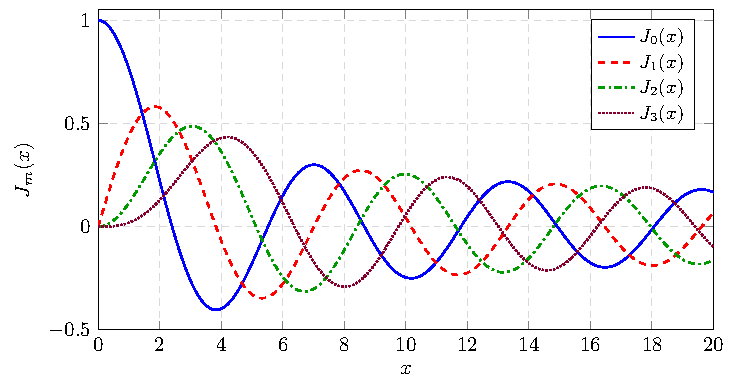
\includegraphics[width=0.86\linewidth]{figs/bessel-J.pdf}
\end{center}
\textbf{Reading the plot.} Near $x=0$, $J_m(x)\approx(x/2)^m/m!$ by \eqref{eq:series}, so
$J_0(0)=1$ and $J_m(0)=0$ for $m\ge1$. In \eqref{eq:bessel-ode-opening} divided by $x^2$, the
term $-m^2/x^2$ acts like a centrifugal barrier: for $x<m$ it prevents oscillation, so
$J_m$ rises slowly from zero and higher angular modes stay away from the center. For large
$x$, each $J_m$ is a slowly decaying cosine with zeros spaced by about $\pi$ (derived under
Asymptotics).
\end{frame}

\begin{frame}[allowframebreaks=1.00]{Jacobi--Anger: the generating function on $|t|=1$}
\footnotesize
Set $t=e^{i\theta}$ in \eqref{eq:genf}. Since $t-t^{-1}=2i\sin\theta$ and
$t^m=e^{im\theta}$,
\begin{equation}
 e^{ix\sin\theta}=\sum_{m=-\infty}^{\infty}J_m(x)e^{im\theta}.
 \label{eq:jacobi-anger}
\end{equation}
This is the Jacobi--Anger expansion, the plane-wave Fourier series that motivated
\eqref{eq:genf}.

To isolate $J_n$, multiply by $e^{-in\theta}$ and integrate over one period, term by
term. For an integer $q$, $\int_0^{2\pi}e^{iq\theta}\,d\theta$ is $2\pi$ if $q=0$ and
$(e^{2\pi iq}-1)/(iq)=0$ otherwise; with $q=m-n$,
\[
 \int_0^{2\pi}e^{ix\sin\theta}e^{-in\theta}\,d\theta
 =\sum_{m=-\infty}^{\infty}J_m(x)\int_0^{2\pi}e^{i(m-n)\theta}\,d\theta
 =2\pi J_n(x),
\]
since only the $m=n$ term survives. Dividing by $2\pi$ and combining the exponentials leaves
\begin{equation}
 J_n(x)=\frac1{2\pi}\int_0^{2\pi}
             e^{i(x\sin\theta-n\theta)}\,d\theta,\qquad n\in\mathbb Z.
 \label{eq:jacobi-anger-coefficient}
\end{equation}
Section~\ref{sec:int-rep} turns this into a real cosine integral. First we use $g$ once more, to
relate neighboring orders.
\end{frame}

% ======================================================================
\section{Recursion formulae}
% ======================================================================

\begin{frame}[allowframebreaks=1.00]{Differentiating in $t$: the three-term recurrence}
\footnotesize
\textbf{Why recurrences?} They give every $J_m$ from $J_0$ and $J_1$, and they turn
$J_m'$ into Bessel functions; the boundary conditions and the Fourier--Bessel norm later
need exactly that.
The goal is a relation among $J_{m-1}$, $J_m$, $J_{m+1}$ and then one for $J_m'$.
Differentiate both sides of the generating function \eqref{eq:genf} in $t$. With $g=e^{x(t-t^{-1})/2}$ and
$\partial_t(t-t^{-1})=1+t^{-2}$, the chain rule gives $g_t=\frac x2(1+t^{-2})g$; termwise differentiation
of the series gives $g_t=\sum_m mJ_m(x)t^{m-1}$. Multiply both by $t$ before comparing coefficients:
\begin{equation}
 tg_t=\frac x2(t+t^{-1})g,
 \qquad tg_t=\sum_{m=-\infty}^{\infty}mJ_m(x)t^m.
 \label{eq:dgdt-A}
\end{equation}
Multiplication by $t$ moves the coefficient of $t^{m-1}$ to $t^m$; multiplication by
$t^{-1}$ moves the coefficient of $t^{m+1}$ to $t^m$. Consequently,
\[
 [t^m](tg)=J_{m-1}(x),\qquad [t^m](t^{-1}g)=J_{m+1}(x).
\]
Matching the coefficient of $t^m$ in \eqref{eq:dgdt-A} gives
\[
 mJ_m(x)=\frac x2\bigl[J_{m-1}(x)+J_{m+1}(x)\bigr].
\]
For $x\ne0$, divide by $x/2$:
\begin{equation}
 J_{m-1}(x)+J_{m+1}(x)=\frac{2m}{x}J_m(x).
 \label{eq:rec1}
\end{equation}
\end{frame}

\begin{frame}[allowframebreaks=1.00]{Differentiating in $x$: the derivative recurrence}
\footnotesize
The $t$-derivative gave the relation among neighboring orders. To express the derivative $J_m'$
itself through neighboring orders, differentiate the same generating function in $x$:
\begin{equation}
 g_x=\tfrac12(t-t^{-1})g,
 \qquad g_x=\sum_{m=-\infty}^{\infty}J_m'(x)t^m.
 \label{eq:dgdx-A}
\end{equation}
Match the coefficient of $t^m$ in \eqref{eq:dgdx-A}. The coefficient shifts are the same as before, with a minus sign between them:
\[
 J_m'(x)=[t^m]g_x=\tfrac12\bigl([t^m](tg)-[t^m](t^{-1}g)\bigr)
 =\tfrac12\bigl[J_{m-1}(x)-J_{m+1}(x)\bigr],
\]
that is,
\begin{equation}
 2J_m'(x)=J_{m-1}(x)-J_{m+1}(x).
 \label{eq:rec2}
\end{equation}
Now add and subtract \eqref{eq:rec1} and \eqref{eq:rec2}:
\[
 2J_{m-1}=\frac{2m}{x}J_m+2J_m',\qquad
 2J_{m+1}=\frac{2m}{x}J_m-2J_m'.
\]
Solving each for $J_m'$ gives, for $x\ne0$,
\begin{align}
 J_m'&=J_{m-1}-\frac m xJ_m,\label{eq:rec-derivative-lower}\\
 J_m'&=\frac m xJ_m-J_{m+1}.\label{eq:rec-derivative-upper}
\end{align}
\end{frame}

\begin{frame}[allowframebreaks=1.00]{Consequences and low-order checks}
\footnotesize
Putting $m=0$ in \eqref{eq:rec-derivative-upper} gives
\begin{equation}
 J_0'(x)=-J_1(x).
 \label{eq:J0-prime}
\end{equation}
One series check, using the low-order series for $J_0$ and $J_1$ from \eqref{eq:series}, confirms the sign:
\[
 \frac{d}{dx}\left(1-\frac{x^2}{4}+\frac{x^4}{64}+\cdots\right)
 =-\frac x2+\frac{x^3}{16}+\cdots=-J_1(x).
\]
The one-sided recurrences also turn products into derivatives. For $x\ne0$,
\begin{align}
 \frac{d}{dx}(x^mJ_m)
 &=x^m\left(J_m'+\frac m xJ_m\right)
 =x^mJ_{m-1},\label{eq:product-rec-lower}\\
 \frac{d}{dx}(x^{-m}J_m)
 &=x^{-m}\left(J_m'-\frac m xJ_m\right)
 =-x^{-m}J_{m+1}.\label{eq:product-rec-upper}
\end{align}
The first equality on each line is the product rule, with $\frac{d}{dx}x^{\pm m}=\pm\frac mx\,x^{\pm m}$; the second uses
\eqref{eq:rec-derivative-lower} and \eqref{eq:rec-derivative-upper}, respectively, rearranged.
Read backwards, the first is an integral, $\int x^mJ_{m-1}\,dx=x^mJ_m+C$; the second returns
for the spherical Bessel functions.
\end{frame}

% ======================================================================
\section{Integral representation}\label{sec:int-rep}
% ======================================================================

\begin{frame}[allowframebreaks=1.00]{Bessel's real integral representation}
\footnotesize
\textbf{Goal.} Write $J_m(x)$ as a real integral over $[0,\pi]$,
\[
 J_m(x)=\frac1\pi\int_0^\pi\cos(m\theta-x\sin\theta)\,d\theta,
\]
which is \eqref{eq:int-rep} below. The route: split the Jacobi--Anger expansion into its real
(cosine) and imaginary (sine) parts, then project each onto the matching Fourier mode on $[0,\pi]$.

\textbf{Step 1: pair the orders \(m\) and \(-m\).} Take \(x\) real, so every \(J_m(x)\) is real. In the
Jacobi--Anger expansion \eqref{eq:jacobi-anger}, group the terms \(m\) and \(-m\) (for \(m\ge1\)). Since
\(J_{-m}=(-1)^mJ_m\) by \eqref{eq:neg-order}, and \(e^{i\phi}\pm e^{-i\phi}\) is \(2\cos\phi\) or \(2i\sin\phi\),
\[
 J_me^{im\theta}+J_{-m}e^{-im\theta}
 =J_m\bigl(e^{im\theta}+(-1)^me^{-im\theta}\bigr)
 =\begin{cases}2J_m\cos(m\theta),&m\text{ even},\\
 2iJ_m\sin(m\theta),&m\text{ odd}.\end{cases}
\]
\textbf{Step 2: real and imaginary parts.} The even orders give real cosine terms, the odd orders give
imaginary sine terms. The left side is \(e^{ix\sin\theta}=\cos(x\sin\theta)+i\sin(x\sin\theta)\). Comparing real
and imaginary parts:
\begin{align*}
 \cos(x\sin\theta)
 &=J_0(x)+2J_2(x)\cos2\theta+2J_4(x)\cos4\theta+\cdots,\\
 \sin(x\sin\theta)
 &=2J_1(x)\sin\theta+2J_3(x)\sin3\theta+\cdots .
\end{align*}
These are ordinary Fourier series in \(\theta\), with the \(J_m\) as coefficients.
\par\framebreak\par
\textbf{Step 3: pick out one coefficient (projection).} Use the integrals on \([0,\pi]\), for
\(j,m\ge1\):
\[
 \int_0^\pi\cos j\theta\cos m\theta\,d\theta=\int_0^\pi\sin j\theta\sin m\theta\,d\theta=\frac\pi2\,\delta_{jm},
\]
together with \(\int_0^\pi\cos m\theta\,d\theta=0\) and \(\int_0^\pi d\theta=\pi\).
\begin{itemize}
  \item \emph{\(m\) even, \(m\ge2\).} Multiply the cosine series by \(\cos m\theta\) and integrate: only the term
        \(2J_m\cos m\theta\) survives, giving \(2J_m\cdot\frac\pi2=\pi J_m\). The sine series contains only odd
        modes, so \(\int_0^\pi\sin(x\sin\theta)\sin m\theta\,d\theta=0\).
  \item \emph{\(m\) odd.} The other way round: \(\int_0^\pi\sin(x\sin\theta)\sin m\theta\,d\theta=\pi J_m\), and the cosine
        integral is \(0\).
  \item \emph{\(m=0\).} \(\int_0^\pi\cos(x\sin\theta)\,d\theta=\pi J_0\), and the sine integral is \(0\) (since
        \(\sin0=0\)).
\end{itemize}
\textbf{Step 4: add the two integrals.} In every case exactly one of them is \(\pi J_m\) and the other is \(0\),
so their sum is \(\pi J_m\):
\[
 \int_0^\pi\bigl[\cos(x\sin\theta)\cos m\theta+\sin(x\sin\theta)\sin m\theta\bigr]\,d\theta=\pi J_m(x).
\]
The bracket is \(\cos(A-B)=\cos A\cos B+\sin A\sin B\) with \(A=m\theta\), \(B=x\sin\theta\). Dividing by \(\pi\), for
\(m\ge0\) (negative orders then follow from \eqref{eq:neg-order}):
\begin{align}
 J_m(x)&=\frac1\pi\int_0^\pi\cos(m\theta-x\sin\theta)\,d\theta,
 \label{eq:int-rep}\\
 J_0(x)&=\frac1\pi\int_0^\pi\cos(x\sin\theta)\,d\theta.
 \label{eq:J0-int}
\end{align}

\textbf{What it buys.} $J_m$ is the average of a cosine over $[0,\pi]$, so $|J_m(x)|\le1$ for
all real $x$, as in the plot. And \eqref{eq:J0-int} shows $J_0$ as the average of $\cos(x\sin\theta)$ over
directions: a superposition of plane waves.
\end{frame}





% ======================================================================
\section{Asymptotics}
% ======================================================================

\begin{frame}[allowframebreaks=1.00]{Small $x$: leading term and first correction}
\footnotesize
\textbf{Why two limits?} Near the axis ($x\to0$) we must know which solutions stay
finite; far out ($x\to\infty$) we need the zeros and the travelling-wave form.
First the small-$x$ limit: the goal is to show $J_m(x)\approx(x/2)^m/m!$ with the next correction.

For fixed $m\ge0$, take the first two terms of \eqref{eq:series} and factor out
$(x/2)^m/m!$, using $(m+1)!=(m+1)m!$:
\[
 J_m(x)=\frac{(x/2)^m}{m!}-\frac{(x/2)^{m+2}}{(m+1)!}+O(x^{m+4})
 =\frac{(x/2)^m}{m!}\left[1-\frac{x^2}{4(m+1)}+O(x^4)\right].
\]
In particular,
\begin{equation}
 J_m(x)=\frac{(x/2)^m}{\Gamma(m+1)}+O(x^{m+2}),\qquad x\to0,
 \label{eq:smallx}
\end{equation}
with the order held fixed. The gamma notation agrees with the general-order series
\eqref{eq:series-gamma}. Since $J_m(0)=0$ for $m\ge1$, on a drum only the
axisymmetric ($m=0$) modes move the centre.
\end{frame}

\begin{frame}[allowframebreaks=1.00]{Large $x$: Bessel functions become slowly decaying waves}
\footnotesize
\textbf{Goal.} Show that for fixed \(m\) and large \(x\), \(J_m\) behaves like a cosine wave whose amplitude
decays like \(1/\sqrt x\):
\[
 J_m(x)\approx\sqrt{\frac{2}{\pi x}}\cos\Bigl(x-\frac{m\pi}{2}-\frac\pi4\Bigr).
\]
\textbf{Idea.} For large \(x\) the term \(\frac1xy'\) in Bessel's equation is a small ``damping''. Remove it
by a change of unknown; what remains is almost the oscillator \(u''+u=0\).

\textbf{Step 1: substitute \(y=x^{-1/2}u\).} By the product rule,
\[
 y'=x^{-1/2}u'-\tfrac12x^{-3/2}u,\qquad
 y''=x^{-1/2}u''-x^{-3/2}u'+\tfrac34x^{-5/2}u .
\]
\par\framebreak\par
\textbf{Step 2: insert into Bessel's equation divided by \(x^2\),}
\(y''+\frac1xy'+\bigl(1-\frac{m^2}{x^2}\bigr)y=0\). The middle term is
\(\frac1xy'=x^{-3/2}u'-\frac12x^{-5/2}u\). Adding the three pieces:
\begin{itemize}
  \item \(u'\) terms: \(-x^{-3/2}u'+x^{-3/2}u'=0\) (the damping is gone);
  \item \(x^{-5/2}u\) terms: \(\bigl(\frac34-\frac12\bigr)x^{-5/2}u=\frac14x^{-5/2}u\);
  \item the rest: \(x^{-1/2}u''+\bigl(1-\frac{m^2}{x^2}\bigr)x^{-1/2}u\).
\end{itemize}
Multiply by \(x^{1/2}\) and collect the \(1/x^2\) terms:
\[
 u''+\Bigl(1-\frac{m^2-\frac14}{x^2}\Bigr)u=0 .
\]
\textbf{Step 3: large \(x\).} The term \((m^2-\frac14)/x^2\) tends to \(0\), so for large \(x\) the equation
is \(u''+u\approx0\), with solutions \(u\approx A\cos(x-\varphi)\) for some amplitude \(A\) and phase \(\varphi\).
Going back, \(y=x^{-1/2}u\):
\[
 J_m(x)\approx\frac{A}{\sqrt x}\cos(x-\varphi).
\]
\textbf{Step 4: the constants} (quoted). The equation alone cannot fix \(A\) and \(\varphi\), because they
depend on which solution we follow from \(x=0\). Evaluating the integral representation
\eqref{eq:int-rep} for large \(x\) gives \(A=\sqrt{2/\pi}\) and \(\varphi=\frac{m\pi}2+\frac\pi4\):
\begin{equation}
 J_m(x)=\sqrt{\frac2{\pi x}}
       \cos\left(x-\frac{m\pi}{2}-\frac\pi4\right)+O(x^{-3/2}),
 \qquad x\to+\infty .
 \label{eq:largex}
\end{equation}
\par\framebreak\par
\textbf{Physical reading.} With \(x=kr\), \(J_m(kr)\) is a standing cylindrical wave whose amplitude falls
like \(1/\sqrt r\): the energy, proportional to amplitude\(^2\), is spread over a circle of length \(2\pi r\),
and \((1/\sqrt r)^2\cdot2\pi r\) is constant.

\textbf{Check.} The first zero of \(\cos(x-\pi/4)\) is at \(x-\pi/4=\pi/2\), i.e.\ \(x=3\pi/4\approx2.36\); the
true first zero of \(J_0\) is \(2.405\). Even this early the formula is off by only about \(2\%\).
\end{frame}


% ======================================================================
\section{Neumann functions}
% ======================================================================

\begin{frame}[allowframebreaks=1.00]{Noninteger order: definition and independence of $Y_\nu$}
\footnotesize
\textbf{Why a second solution?} On a full disk $J_m$ suffices. But when the origin is
not in the region (an annulus, a coaxial cable, the outside of a cylinder in
scattering), the radial solution needs a second, independent function, and the
combinations $J\pm iY$ of the next section are the outgoing and incoming waves.
Chapter~3, \S3.3 built one by reduction of order,
$\widetilde Y_m=J_m\int_{x_*}^{x}ds/[sJ_m^2(s)]$, singular at $x=0$, but its scale and its
added multiple of $J_m$ were arbitrary. We now fix one standard choice for every real order.

For $x>0$, dividing Bessel's equation \eqref{eq:bessel-ode-opening} by $x^2$ gives
\begin{equation}
 y''+\frac1x y'+\left(1-\frac{m^2}{x^2}\right)y=0.
 \label{eq:bessel-normal-form}
\end{equation}
\textbf{Two solutions for noninteger \(\nu\).} With \(m\) replaced by a real order \(\nu\), the equation contains
the order only through \(\nu^2\). The series \eqref{eq:series-gamma} solves it (Chapter~3, root \(r=\nu\)). Changing
\(\nu\) to \(-\nu\) does not change \(\nu^2\), so \(J_{-\nu}(x)\) is a solution too.

\textbf{Definition.} For fixed real \(\nu\notin\mathbb Z\), define
\begin{equation}
  Y_\nu(x)=
  \frac{J_\nu(x)\cos(\pi\nu)-J_{-\nu}(x)}{\sin(\pi\nu)}.
  \label{eq:neumann-def}
\end{equation}
\textbf{Why this particular combination?} Two reasons. (1) At integer \(\nu\), both numerator and
denominator become zero, so the limit can be finite; this gives \(Y_m\) for integer order (next frame).
(2) At large \(x\), it turns \(J_\nu\)'s cosine into a sine (end of this section).

\par\framebreak\par
\textbf{Independence: compute the Wronskian.}

\emph{Step 1: it has the form \(C/x\).} For \eqref{eq:bessel-normal-form}, \(P=1/x\). By Abel's identity
(Chapter~3), the Wronskian of any two solutions is \(C\,e^{-\int dx/x}=C\,e^{-\ln x}=C/x\). So we only need the
constant \(C\), and the leading terms near \(x=0\) are enough to find it (the corrections bring higher
powers of \(x\), which cannot affect the \(1/x\) term).

\emph{Step 2: the leading terms.} \(J_{\pm\nu}\approx\frac{(x/2)^{\pm\nu}}{\Gamma(1\pm\nu)}\). For the two powers,
using \(\frac{d}{dx}(x/2)^{\pm\nu}=\pm\frac\nu x(x/2)^{\pm\nu}\),
\[
 W\bigl[(x/2)^{\nu},(x/2)^{-\nu}\bigr]
 =(x/2)^\nu\cdot\Bigl(-\frac\nu x\Bigr)(x/2)^{-\nu}-\frac\nu x(x/2)^\nu\cdot(x/2)^{-\nu}
 =-\frac{2\nu}{x}.
\]
\par\framebreak\par
\emph{Step 3: include the constants and simplify.} Divide by \(\Gamma(1+\nu)\Gamma(1-\nu)\). Since
\(\Gamma(1+\nu)=\nu\,\Gamma(\nu)\) and, by the reflection formula (Chapter~2),
\(\Gamma(\nu)\Gamma(1-\nu)=\pi/\sin(\pi\nu)\):
\[
 W[J_\nu,J_{-\nu}]=\frac{-2\nu}{\Gamma(1+\nu)\,\Gamma(1-\nu)\,x}
 =\frac{-2\nu}{\nu\,\Gamma(\nu)\Gamma(1-\nu)\,x}
 =-\frac{2\sin(\pi\nu)}{\pi x}.
\]
\emph{Step 4: the Wronskian of \(J_\nu\) and \(Y_\nu\).} The Wronskian is linear in each slot, and
\(W[J_\nu,J_\nu]=0\). By \eqref{eq:neumann-def},
\[
 W[J_\nu,Y_\nu]=\frac{\cos(\pi\nu)\,W[J_\nu,J_\nu]-W[J_\nu,J_{-\nu}]}{\sin(\pi\nu)}
 =\frac{0+\frac{2\sin(\pi\nu)}{\pi x}}{\sin(\pi\nu)}=\frac{2}{\pi x}\ne0,
\]
so \(J_\nu\) and \(Y_\nu\) are independent. (This is the normalization \(2/(\pi x)\) already met in Chapter~3.)
\end{frame}

\begin{frame}[allowframebreaks=1.00]{Integer order: define the second solution by a limit}
\footnotesize
At an integer $m$, $J_{-m}=(-1)^mJ_m$ by \eqref{eq:neg-order}, $\cos(\pi m)=(-1)^m$, and
$\sin(\pi m)=0$. Thus direct substitution into \eqref{eq:neumann-def} gives $0/0$,
not a value for $Y_m$.

The conventional definition is the continuous limit
\begin{equation}
 Y_m(x)=\lim_{\nu\to m}
 \frac{J_\nu(x)\cos(\pi\nu)-J_{-\nu}(x)}{\sin(\pi\nu)},\qquad x>0.
 \label{eq:Y-integer-limit}
\end{equation}
This limit exists and still solves the integer-order Bessel equation (standard result).
The Wronskian passes to the limit:
\begin{equation}
 W[J_m,Y_m]=\frac2{\pi x}\ne0.
 \label{eq:JY-wronskian}
\end{equation}
So $Y_m$ is independent of $J_m$, even though $J_{-m}$ is not.

\textbf{Link to Chapter~3.} There, $W[J_m,\widetilde Y_m]=1/x$; matching this with
\eqref{eq:JY-wronskian} gave
\begin{equation}
 Y_m=\frac2\pi\,\widetilde Y_m+C\,J_m .
 \label{eq:Y-from-Ytilde}
\end{equation}
The Wronskian fixed the factor $2/\pi$; the limit \eqref{eq:Y-integer-limit} also fixes the constant $C$.
\end{frame}

\begin{frame}{Bessel functions of the second kind}
\footnotesize
\begin{center}
  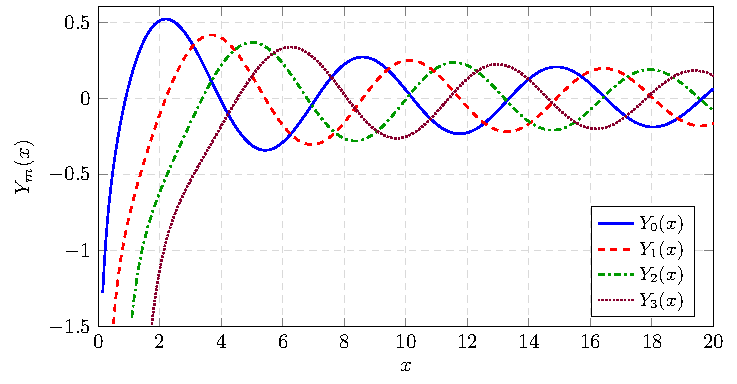
\includegraphics[width=0.86\linewidth]{figs/bessel-Y.pdf}
\end{center}
The Neumann functions are independent of $J_m$ and singular at $x=0$. For large positive
$x$, $J_m$ and $Y_m$ have the same $x^{-1/2}$ envelope and phases shifted by $\pi/2$
(see \eqref{eq:Jlarge}--\eqref{eq:Ylarge} below).
\end{frame}

\begin{frame}[allowframebreaks=1.00]{Small-$x$ behavior of $Y_m$}
\footnotesize
\textbf{Why we need it.} Chapter~3 showed that $Y_m$ blows up at the origin, which is why
disk modes exclude it. Here we find the exact leading constants that Chapter~3 left open,
and the noninteger formula \eqref{eq:Ysmall-general} that gives $y_n$ for small $x$ at the
end of the chapter.

First let $\nu>0$ be fixed and noninteger. From the $k=0$ term of \eqref{eq:series-gamma}
(used once with order $\nu$ and once with order $-\nu$),
\[
  J_{\pm\nu}(x)=\frac{1}{\Gamma(1\pm\nu)}\left(\frac{x}{2}\right)^{\pm\nu}[1+O(x^2)].
\]
Since $x^\nu/x^{-\nu}=x^{2\nu}\to0$, the $J_{-\nu}$ term dominates in
\eqref{eq:neumann-def}. Therefore, writing $[1+o(1)]$ for a factor that tends to $1$,
\[
  Y_\nu(x)
  =-\frac{1}{\Gamma(1-\nu)\sin(\pi\nu)}
  \left(\frac{x}{2}\right)^{-\nu}[1+o(1)].
\]
Euler's reflection formula (Chapter~2) gives
\[
 \Gamma(\nu)\Gamma(1-\nu)=\frac\pi{\sin(\pi\nu)}
 \quad\Longrightarrow\quad
 \frac1{\Gamma(1-\nu)\sin(\pi\nu)}=\frac{\Gamma(\nu)}\pi.
\]
Consequently,
\begin{equation}
  Y_\nu(x)=-\frac{\Gamma(\nu)}{\pi}
  \left(\frac{2}{x}\right)^\nu[1+o(1)],
  \qquad x\to0^+,
  \label{eq:Ysmall-general}
\end{equation}
for fixed positive noninteger $\nu$.

\par\framebreak\par
For integer $m\ge1$, Chapter~3 found $\widetilde Y_m(x)\sim-2^{m-1}(m-1)!\,x^{-m}$ as $x\to0^+$. In
\eqref{eq:Y-from-Ytilde} the term $CJ_m=O(x^m)$ is negligible, so
\begin{equation}
 Y_m(x)=\frac2\pi\Bigl[-2^{m-1}(m-1)!\,x^{-m}\Bigr][1+o(1)]
 =-\frac{\Gamma(m)}{\pi}\left(\frac2x\right)^m[1+o(1)],
 \label{eq:Ysmall}
\end{equation}
the same as letting $\nu\to m$ in \eqref{eq:Ysmall-general}.

For $m=0$, Chapter~3 found $\widetilde Y_0=\ln x+\text{const}+\cdots$ (the integrand is
$1/[sJ_0^2(s)]=1/s+O(s)$), so $Y_0=\frac2\pi\ln x+\text{const}$. The limit
definition fixes the constant (quoted, DLMF \S10.8):
\begin{equation}
 Y_0(x)=\frac2\pi\left[\ln\left(\frac x2\right)+\gamma\right]
       +O(x^2|\ln x|),\qquad x\to0^+,
 \label{eq:Y0-small}
\end{equation}
where $\gamma\approx0.5772$ is the Euler--Mascheroni constant of Chapter~2.
\end{frame}

\begin{frame}[allowframebreaks=1.00]{Large-$x$ behavior of $J_\nu$ and $Y_\nu$}
\footnotesize
\textbf{Goal.} Find the large-$x$ form of $Y_\nu$, given the cosine law for $J_\nu$ and the
definition \eqref{eq:neumann-def} of $Y_\nu$ as a combination of $J_{\nu}$ and $J_{-\nu}$.
The expected result is the same amplitude with a sine in place of the cosine.

For fixed real order $\nu$, set
\[
 \chi_\nu(x)=x-\frac{\nu\pi}{2}-\frac\pi4,\qquad A(x)=\sqrt{\frac2{\pi x}}.
\]
The cosine law \eqref{eq:largex} also holds for fixed noninteger $\nu$ (quoted, DLMF
\S10.17):
\begin{equation}
 J_\nu(x)=A(x)\cos\chi_\nu(x)+O(x^{-3/2}).
 \label{eq:Jlarge}
\end{equation}
\par\framebreak\par
Since $\chi_{-\nu}=x+\frac{\nu\pi}2-\frac\pi4=\chi_\nu+\pi\nu$, insert \eqref{eq:Jlarge} for $J_\nu$ and $J_{-\nu}$ into the
definition \eqref{eq:neumann-def} of $Y_\nu$ for fixed noninteger $\nu$:
\[
 Y_\nu(x)=A(x)\frac{\cos\chi_\nu\cos(\pi\nu)-\cos(\chi_\nu+\pi\nu)}
                         {\sin(\pi\nu)}+O(x^{-3/2}).
\]
The identity $\cos(\chi+\beta)=\cos\chi\cos\beta-\sin\chi\sin\beta$ makes the numerator
$\sin\chi_\nu\sin(\pi\nu)$, so
\begin{equation}
 Y_\nu(x)=\sqrt{\frac2{\pi x}}\sin\chi_\nu(x)+O(x^{-3/2}),
 \qquad x\to+\infty.
 \label{eq:Ylarge}
\end{equation}
The same sine law holds at integer order (quoted; DLMF \S10.17). Thus $J_m$ and $Y_m$
behave like $\cos$ and $\sin$ of the same phase, with the same envelope; the next section
combines them into travelling waves.
\end{frame}

% ======================================================================
\section{Hankel functions and Fourier--Bessel series}
% ======================================================================

\begin{frame}[allowframebreaks=1.00]{Hankel functions: Bessel functions of the third kind}
\footnotesize
\textbf{Why?} Far away, $J_m$ and $Y_m$ behave like $\cos$ and $\sin$ by \eqref{eq:Jlarge} and
\eqref{eq:Ylarge}: standing waves. A source that radiates, or a wave that is scattered,
needs a \emph{travelling} wave, so we combine them as in $\cos\chi\pm i\sin\chi=e^{\pm i\chi}$:
\begin{align}
  H_m^{(1)}(x)&=J_m(x)+iY_m(x),
  \label{eq:hankel1}\\
  H_m^{(2)}(x)&=J_m(x)-iY_m(x).
  \label{eq:hankel2}
\end{align}
With $\chi_m(x)=x-\frac{m\pi}{2}-\frac{\pi}{4}$, the two large-$x$ laws give
\[
  H_m^{(1,2)}(x)
  =\sqrt{\frac{2}{\pi x}}
    \bigl(\cos\chi_m\pm i\sin\chi_m\bigr)+O(x^{-3/2})
  =\sqrt{\frac{2}{\pi x}}\,e^{\pm i\chi_m(x)}+O(x^{-3/2}).
\]
With $k>0$, $\omega>0$, and time dependence $e^{-i\omega t}$,
\[
 H_m^{(1)}(kr)e^{-i\omega t}
 \sim \sqrt{\frac{2}{\pi kr}}\,
 e^{i(kr-\omega t-m\pi/2-\pi/4)},\qquad r\to\infty
\]
for fixed $m$. On a constant-phase surface $kr-\omega t=\text{const}$; differentiating in $t$ gives
$dr/dt=\omega/k>0$, so the surfaces move toward larger $r$: the wave is outgoing.
For $H_m^{(2)}(kr)e^{-i\omega t}$ the phase is $-(kr+\omega t)$ up to a constant, so
$dr/dt=-\omega/k<0$: incoming. The Hankel functions are exact solutions for $r>0$ (only
the exponential forms are far-field approximations), and both are singular at the origin.
\end{frame}

\begin{frame}{Discrete radial modes on the unit disk}
\footnotesize
\begin{center}
  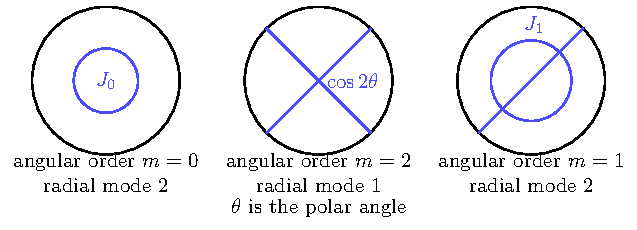
\includegraphics[width=0.78\linewidth]{figs/bessel_disk_modes.pdf}
\end{center}
Here $\alpha_{m,j}$ is the $j$th positive zero of $J_m$ (Chapter~3's $\alpha_{m,n}$): the
condition $J_m(\alpha_{m,j})=0$ puts a radial node on the clamped rim $r=1$. There are
infinitely many zeros $\alpha_{m,1}<\alpha_{m,2}<\cdots$, because the cosine law
\eqref{eq:largex} changes sign again and again; each is simple, since at $J_m(a)=0$ the
Wronskian \eqref{eq:JY-wronskian} reduces to $-J_m'(a)Y_m(a)=2/(\pi a)\ne0$.

\textbf{Physical meaning.} For a membrane with wave speed $c$, the frequency is $\omega=ck$,
and the rim condition $J_m(k\cdot1)=0$ forces $k=\alpha_{m,j}$. So the drum's axisymmetric
($m=0$) frequencies are proportional to $\alpha_{0,j}=2.405,\ 5.520,\ 8.654,\ldots$,
in ratios $1:2.30:3.60$. A string's are $1:2:3$; a drum's overtones are not harmonic.
\end{frame}

\begin{frame}[allowframebreaks=1.00]{Drum modes: orthogonality}
\footnotesize
We want to expand a drum shape in these modes, so we need their orthogonality and norms.
Precisely, we will show that for the positive zeros $\alpha_{m,j}$ of $J_m$,
\[
 \int_0^1xJ_m(\alpha_{m,j}x)J_m(\alpha_{m,k}x)\,dx=\frac12J_{m+1}^2(\alpha_{m,j})\,\delta_{jk};
\]
this frame does the case $j\ne k$ and the next the case $j=k$.
Chapter~4's drum example put $y(x)=J_m(\alpha x)$, $0\le x\le1$, in Sturm--Liouville form:
\begin{equation}
 (xy')'-\frac{m^2}{x}y=-\alpha^2x\,y,
 \label{eq:sl}
\end{equation}
so $p=w=x$, $q=-m^2/x$, $\lambda=\alpha^2$. The weight has a picture: $x\,dx\,d\theta$ is the
area element of the disk, so orthogonality with weight $x$ is ordinary orthogonality over the
drum's area. Chapter~4 also showed that the boundary term $x(uv'-u'v)$ vanishes at $x=0$ for
regular modes (for a singular $Y_m$ it would not) and at the rim, where
the modes vanish. We redo the cross integral only because its limit $b\to a$ gives the norm.

For $a,b>0$ let $y_a(x)=J_m(ax)$ and $y_b(x)=J_m(bx)$; each solves \eqref{eq:sl} with
$\alpha=a$ or $b$. Chapter~4's integrated Green identity with $p=w=x$, $\lambda=a^2,b^2$ (all
real), and the vanishing term at $x=0$, gives, since $y_a(1)=J_m(a)$ and $y_a'(1)=aJ_m'(a)$,
\[
 (a^2-b^2)\int_0^1xy_ay_b\,dx=\bigl[x(y_ay_b'-y_a'y_b)\bigr]_{x=1}
 =bJ_m(a)J_m'(b)-aJ_m'(a)J_m(b).
\]
Dividing by $a^2-b^2$ gives
\begin{equation}
 \int_0^1xJ_m(ax)J_m(bx)\,dx
 =\frac{bJ_m(a)J_m'(b)-aJ_m(b)J_m'(a)}{a^2-b^2},\quad a\ne b.
 \label{eq:bessel-cross-integral}
\end{equation}
Now choose distinct positive zeros $a=\alpha_{m,j}$ and $b=\alpha_{m,k}$ of $J_m$.
Both $J_m(a)$ and $J_m(b)$ are zero, so the numerator vanishes while $a^2-b^2\ne0$:
\begin{equation}
 \int_0^1xJ_m(\alpha_{m,j}x)J_m(\alpha_{m,k}x)\,dx=0,
 \qquad j\ne k.
 \label{eq:bessel-orth-offdiag}
\end{equation}
For the diagonal case $j=k$, both numerator and denominator vanish instead.
We therefore take a limit, rather than substitute $a=b$ into \eqref{eq:bessel-cross-integral}.
\end{frame}

\begin{frame}[allowframebreaks=1.00]{Fourier--Bessel normalization: the diagonal case}
\footnotesize
To compute the norm at a positive zero $a$ of $J_m$, let $b\to a$ in
\eqref{eq:bessel-cross-integral}; the left side tends to $\int_0^1xJ_m^2(ax)\,dx$.
With $a$ fixed and $J_m(a)=0$, the numerator and denominator are
\[
  N(b)=bJ_m(a)J_m'(b)-aJ_m(b)J_m'(a)=-aJ_m(b)J_m'(a),\qquad D(b)=a^2-b^2.
\]
Both vanish at $b=a$, a $0/0$ form. L'H\^opital in $b$, with
$N'(b)=-aJ_m'(b)J_m'(a)$ and $D'(b)=-2b$, gives
\begin{equation}
  \int_0^1xJ_m^2(ax)\,dx=\lim_{b\to a}\frac{N(b)}{D(b)}
  =\frac{N'(a)}{D'(a)}
  =\frac{-aJ_m'(a)J_m'(a)}{-2a}
  =\frac12\bigl[J_m'(a)\bigr]^2,
  \label{eq:bessel-norm-prime}
\end{equation}
nonzero because the zero $a$ is simple. At a zero the derivative recurrence
\eqref{eq:rec-derivative-upper} gives $J_m'(a)=\frac{m}{a}J_m(a)-J_{m+1}(a)=-J_{m+1}(a)$,
and squaring removes the sign. With the off-diagonal case \eqref{eq:bessel-orth-offdiag}:
\begin{equation}
  \int_0^1J_m(\alpha_{m,j}x)J_m(\alpha_{m,k}x)x\,dx
  =\frac12J_{m+1}^2(\alpha_{m,j})\delta_{jk}.
  \label{eq:bessel-orth}
\end{equation}
\end{frame}

\begin{frame}[allowframebreaks=1.00]{Fourier--Bessel coefficients}
\footnotesize
For a radial function of fixed angular order $m$, write
\begin{equation}
 f(x)=\sum_{j=1}^{\infty}a_jJ_m(\alpha_{m,j}x),\qquad 0<x<1.
 \label{eq:fourier-bessel}
\end{equation}
As for the sine series in Chapter~4, equality means convergence in the weighted
mean-square norm $\|g\|^2=\int_0^1|g(x)|^2x\,dx$.

As for the sine series, multiply by the $k$th mode and the weight $x$,
then integrate. Orthogonality \eqref{eq:bessel-orth-offdiag} removes every term except $j=k$,
and \eqref{eq:bessel-orth} evaluates the surviving norm:
\begin{align*}
 \int_0^1 f(x)J_m(\alpha_{m,k}x)x\,dx
 &=\sum_{j=1}^{\infty}a_j\int_0^1J_m(\alpha_{m,j}x)J_m(\alpha_{m,k}x)x\,dx\\
 &=a_k\int_0^1J_m^2(\alpha_{m,k}x)x\,dx
 =\frac{a_k}{2}J_{m+1}^2(\alpha_{m,k}).
\end{align*}
Solving for $a_k$ gives
\begin{equation}
 a_k=\frac{2}{J_{m+1}^2(\alpha_{m,k})}
       \int_0^1f(x)J_m(\alpha_{m,k}x)x\,dx.
 \label{eq:fourier-bessel-coeff}
\end{equation}
The modes are complete (a quoted Sturm--Liouville result): no radial shape with finite
$\int_0^1|f|^2x\,dx$ is missed, just as for the sine series.

\textbf{Example: $f=1$, $m=0$.} Put $t=\alpha_kx$ ($\alpha_k=\alpha_{0,k}$) and use
$\frac{d}{dt}(tJ_1)=tJ_0$, i.e.\ \eqref{eq:product-rec-lower} at $m=1$:
\[
 \int_0^1J_0(\alpha_kx)\,x\,dx=\frac1{\alpha_k^2}\int_0^{\alpha_k}tJ_0(t)\,dt
 =\frac{1}{\alpha_k^2}\bigl[tJ_1(t)\bigr]_0^{\alpha_k}=\frac{J_1(\alpha_k)}{\alpha_k},
 \qquad
 a_k=\frac{2}{\alpha_kJ_1(\alpha_k)}.
\]
Numerically $a_1,a_2,a_3=1.602,\,-1.065,\,0.851$. They decay slowly because $f=1$ does not
vanish at the rim where every mode does, like the sine series of $f=1$ in Chapter~4.
\end{frame}

% ======================================================================
\section{Half-integer order: spherical Bessel functions}
% ======================================================================

\begin{frame}[allowframebreaks=1.00]{The three-dimensional radial equation}
\footnotesize
\textbf{Goal.} Show that the radial equation for waves in three dimensions is Bessel's
equation of half-integer order $n+\tfrac12$, which defines the spherical Bessel functions.

Waves in three dimensions (sound from a small source, scattering by a sphere) obey the
Helmholtz equation $(\nabla^2+k^2)\psi=0$. In spherical coordinates the radial part of
$\nabla^2$ is $r^{-2}(r^2R')'$ (the full Laplacian is written out in Chapter~6), and the angular
part contributes $-n(n+1)/r^2$, $n=0,1,2,\ldots$ (the Legendre eigenvalue of Chapters~4 and~6).
So $\psi=R(r)\times(\text{angular part})$ needs
\[
 \frac1{r^2}(r^2R')'+\Bigl[k^2-\frac{n(n+1)}{r^2}\Bigr]R=0.
\]
\textbf{Step 1: scale.} Multiply by \(r^2\) and put \(x=kr\) (so \(r\frac{d}{dr}=x\frac{d}{dx}\)); with
\((r^2R')'=r^2R''+2rR'\):
\[
 x^2R''+2xR'+\bigl[x^2-n(n+1)\bigr]R=0.
\]
This is almost Bessel's equation, but the middle term is \(2xR'\) instead of \(xR'\).

\textbf{Step 2: remove the extra \(xR'\).} Try \(R=x^{-1/2}w\) (a power of \(x\) times a new function; the power
\(-\frac12\) is the one that works). By the product rule,
\[
 R'=x^{-1/2}w'-\tfrac12x^{-3/2}w,\qquad
 R''=x^{-1/2}w''-x^{-3/2}w'+\tfrac34x^{-5/2}w .
\]
Multiply by \(x^2\) and by \(2x\) and add:
\[
 x^2R''=x^{3/2}w''-x^{1/2}w'+\tfrac34x^{-1/2}w,\qquad
 2xR'=2x^{1/2}w'-x^{-1/2}w,
\]
\[
 x^2R''+2xR'=x^{3/2}w''+x^{1/2}w'-\tfrac14x^{-1/2}w .
\]
\par\framebreak\par
\textbf{Step 3: Bessel's equation appears.} Insert this into Step~1 together with
\(\bigl[x^2-n(n+1)\bigr]R=\bigl[x^2-n(n+1)\bigr]x^{-1/2}w\), and multiply everything by \(x^{1/2}\):
\[
 x^2w''+xw'-\tfrac14w+\bigl[x^2-n(n+1)\bigr]w=0 .
\]
Since \(n(n+1)+\tfrac14=n^2+n+\tfrac14=(n+\tfrac12)^2\), this is Bessel's equation of order \(n+\frac12\):
\[
 x^2w''+xw'+\bigl[x^2-(n+\tfrac12)^2\bigr]w=0.
\]
So $w=J_{n+1/2}$ or $Y_{n+1/2}$, and
$R=x^{-1/2}J_{n+1/2}$ or $x^{-1/2}Y_{n+1/2}$. With the constant
$\sqrt{\pi/2}$ chosen so that $j_0(x)\to1$ as $x\to0^+$ (next slide), the regular and
singular radial solutions are the \emph{spherical Bessel functions}
\begin{equation}
 j_n(x)=\sqrt{\frac{\pi}{2x}}\,J_{n+1/2}(x),\qquad
 y_n(x)=\sqrt{\frac{\pi}{2x}}\,Y_{n+1/2}(x),
 \label{eq:spherical-jy}
\end{equation}
and, with $H_\nu^{(1,2)}=J_\nu\pm iY_\nu$ as in \eqref{eq:hankel1}--\eqref{eq:hankel2}, the
outgoing and incoming waves are the \emph{spherical Hankel functions}
\begin{equation}
 h_n^{(1)}=j_n+iy_n=\sqrt{\frac{\pi}{2x}}H_{n+1/2}^{(1)},\qquad
 h_n^{(2)}=j_n-iy_n=\sqrt{\frac{\pi}{2x}}H_{n+1/2}^{(2)}.
 \label{eq:spherical-h}
\end{equation}
\end{frame}

\begin{frame}[allowframebreaks=1.00]{Elementary functions at half-integer order}
\footnotesize
\textbf{Goal.} At half-integer order the Bessel family reduces to elementary functions. Find \(j_0,y_0\),
then \(j_1,y_1\), and the behaviour of \(j_n,y_n,h_n\) for large and small \(x\).

\textbf{Step 1: solve the case \(n=0\) directly.} The radial equation is \(x^2R''+2xR'+x^2R=0\). Put \(u=xR\).
Then \(u'=R+xR'\) and \(u''=2R'+xR''\), so \(x\,u''=x^2R''+2xR'\). The equation becomes
\[
 x\,u''+x\cdot(xR)=x\,(u''+u)=0
 \quad\Longrightarrow\quad u''+u=0
 \quad\Longrightarrow\quad u=A\sin x+B\cos x .
\]
\textbf{Step 2: which combination is \(j_0\)?} By \eqref{eq:spherical-jy}, \(u=xj_0=\sqrt{\pi x/2}\,J_{1/2}\). Near \(0\),
\(J_{1/2}\approx\frac{(x/2)^{1/2}}{\Gamma(3/2)}\) with \(\Gamma(\frac32)=\frac{\sqrt\pi}2\), so
\[
 u\approx\sqrt{\frac{\pi x}{2}}\cdot\sqrt{\frac x2}\cdot\frac{2}{\sqrt\pi}=x .
\]
\(\sin x\approx x\) and \(\cos x\approx1\) near \(0\), so \(A=1\), \(B=0\): \(u=\sin x\).

\textbf{Step 3: which combination is \(y_0\)?} At \(\nu=\frac12\), \eqref{eq:neumann-def} gives
\(Y_{1/2}=\frac{J_{1/2}\cos\frac\pi2-J_{-1/2}}{\sin\frac\pi2}=-J_{-1/2}\). So \(u=xy_0=-\sqrt{\pi x/2}\,J_{-1/2}\), and with
\(J_{-1/2}\approx\frac{(x/2)^{-1/2}}{\Gamma(1/2)}\), \(\Gamma(\frac12)=\sqrt\pi\):
\[
 u\approx-\sqrt{\frac{\pi x}{2}}\cdot\sqrt{\frac2x}\cdot\frac{1}{\sqrt\pi}=-1
 \quad\Longrightarrow\quad u=-\cos x .
\]
\par\framebreak\par
\textbf{Result for \(n=0\).} Dividing by \(x\),
\[
 j_0(x)=\frac{\sin x}{x},\qquad y_0(x)=-\frac{\cos x}{x}.
\]
For the Hankel functions, use \(\sin x-i\cos x=-i(\cos x+i\sin x)=-ie^{ix}\) and
\(\sin x+i\cos x=i(\cos x-i\sin x)=ie^{-ix}\):
\[
 h_0^{(1)}=j_0+iy_0=\frac{\sin x-i\cos x}{x}=\frac{-i\,e^{ix}}{x},\qquad
 h_0^{(2)}=j_0-iy_0=\frac{i\,e^{-ix}}{x}.
\]
\textbf{In words.} \(xj_0=\sin x=\frac{e^{ix}-e^{-ix}}{2i}\) is a \emph{standing} wave: an outgoing and an incoming
spherical wave of equal strength. Each \(h_0^{(1,2)}\) is a single \emph{traveling} spherical wave, just as
for the cylindrical Hankel functions.
\par\framebreak\par
\textbf{Step 4: higher orders from a recurrence.} The product recurrence \eqref{eq:product-rec-upper},
\(\frac{d}{dx}(x^{-\nu}J_\nu)=-x^{-\nu}J_{\nu+1}\), also holds for noninteger \(\nu\) and for \(Y\) (quoted). At \(\nu=\frac12\),
multiplied by \(\sqrt{\pi/2}\), it says \(j_0'=-j_1\); likewise \(y_0'=-y_1\). So
\[
 j_1=-\frac{d}{dx}\frac{\sin x}{x}=-\frac{x\cos x-\sin x}{x^2}=\frac{\sin x}{x^2}-\frac{\cos x}{x},
\]
\[
 y_1=\frac{d}{dx}\frac{\cos x}{x}=\frac{-x\sin x-\cos x}{x^2}=-\frac{\cos x}{x^2}-\frac{\sin x}{x}.
\]
\textbf{Step 5: the far field.} Insert the Hankel asymptotics \(H^{(1,2)}_\nu\approx\sqrt{2/(\pi x)}\,e^{\pm i\chi_\nu}\) (Hankel
slide) at \(\nu=n+\frac12\) into \eqref{eq:spherical-h}. Three simplifications:
\[
 \chi_{n+1/2}=x-\frac{(n+\frac12)\pi}2-\frac\pi4=x-\frac{(n+1)\pi}{2},
\]
\[
 \sqrt{\frac{\pi}{2x}}\sqrt{\frac{2}{\pi x}}=\frac1x,\qquad
 e^{\mp i(n+1)\pi/2}=(\mp i)^{n+1}.
\]
\par\framebreak\par
So the leading terms are
\begin{equation}
 h_n^{(1)}(x)\approx\frac{(-i)^{n+1}e^{ix}}{x},\qquad
 h_n^{(2)}(x)\approx\frac{i^{n+1}e^{-ix}}{x},\qquad x\to+\infty.
 \label{eq:spherical-h-far}
\end{equation}
The \(1/x\) envelope is spherical spreading (energy \(\propto\) amplitude\(^2\propto1/x^2\), spread over a sphere of
area \(\propto x^2\)), the analogue of the \(1/\sqrt x\) envelope of the cylindrical \(H_m^{(1,2)}\).

\textbf{Convention flag.} With this chapter's time factor \(e^{-i\omega t}\), \(h_n^{(1)}\) and \(H_\nu^{(1)}\) are outgoing;
with \(e^{+i\omega t}\), common in applied scattering, \(h_n^{(2)}\) and \(H_\nu^{(2)}\) are. Always state the time
convention with a Hankel label.

\textbf{Step 6: small argument} (\(x\to0^+\), \(n\) fixed). First a gamma value: applying \(\Gamma(a+1)=a\Gamma(a)\)
repeatedly from \(\Gamma(\frac12)=\sqrt\pi\),
\[
 \Gamma\bigl(n+\tfrac32\bigr)=\tfrac{2n+1}{2}\cdot\tfrac{2n-1}{2}\cdots\tfrac12\cdot\sqrt\pi=\frac{(2n+1)!!}{2^{n+1}}\sqrt\pi,
\]
where \((2n+1)!!=1\cdot3\cdot5\cdots(2n+1)\);
and in the same way \(\Gamma(n+\frac12)=\frac{(2n-1)!!}{2^n}\sqrt\pi\) (with \((-1)!!=1\)).
\par\framebreak\par
\textbf{Step 6, continued.} Multiply the leading terms of \eqref{eq:series-gamma} and \eqref{eq:Ysmall-general} by
\(\sqrt{\pi/(2x)}\), and simplify the powers of \(2\) and \(x\):
\begin{align*}
 j_n(x)&\approx\sqrt{\frac{\pi}{2x}}\,\frac{(x/2)^{n+1/2}}{\Gamma(n+\tfrac32)}
 =\frac{\sqrt\pi\,x^n}{2^{n+1}\,\Gamma(n+\tfrac32)}=\frac{x^n}{(2n+1)!!},\\
 y_n(x)&\approx-\sqrt{\frac{\pi}{2x}}\,\frac{\Gamma(n+\tfrac12)}{\pi}\Bigl(\frac2x\Bigr)^{n+1/2}
 =-\frac{2^n\,\Gamma(n+\tfrac12)}{\sqrt\pi\,x^{n+1}}=-\frac{(2n-1)!!}{x^{n+1}}.
\end{align*}
Check with \(n=0\): \(j_0\approx1\) and \(y_0\approx-1/x\), as from \(\sin x/x\) and \(-\cos x/x\).
\end{frame}

% ======================================================================
\section{Summary}
% ======================================================================

\begin{frame}[allowframebreaks=1.00]{Formula sheet: $J_m$}
\footnotesize

For integer $m\ge0$,
\begin{align*}
  &x^2J_m''(x)+xJ_m'(x)+(x^2-m^2)J_m(x)=0,\\[3pt]
  &J_m(x)=\sum_{k=0}^{\infty}
  \frac{(-1)^k}{k!(m+k)!}\left(\frac{x}{2}\right)^{2k+m},\\[3pt]
  &J_{-m}(x)=(-1)^mJ_m(x).
\end{align*}
The generating function, valid for $t\ne0$, is
\[
  e^{\frac{x}{2}(t-t^{-1})}
  =\sum_{m=-\infty}^{\infty}J_m(x)t^m.
\]
The recurrences are
\begin{align*}
  J_{m-1}(x)+J_{m+1}(x)&=\frac{2m}{x}J_m(x),\qquad x\ne0,\\
  2J_m'(x)&=J_{m-1}(x)-J_{m+1}(x),\\
  J_m'(x)&=J_{m-1}(x)-\frac{m}{x}J_m(x),\qquad x\ne0,\\
  J_m'(x)&=\frac{m}{x}J_m(x)-J_{m+1}(x),\qquad x\ne0.
\end{align*}
The integral representations are
\begin{align*}
  J_m(x)&=\frac{1}{\pi}\int_0^\pi
  \cos(m\theta-x\sin\theta)\,d\theta,
  &&m\ge0,\\
  J_n(x)&=\frac{1}{2\pi}\int_0^{2\pi}
  e^{i(x\sin\theta-n\theta)}\,d\theta,
  &&n\in\mathbb Z,
\end{align*}
For fixed $m$,
\begin{align*}
  J_m(x)
  &=\frac{1}{m!}\left(\frac{x}{2}\right)^m
  \left[1-\frac{x^2}{4(m+1)}+O(x^4)\right],
  &&x\to0,\\
  J_m(x)
  &=\sqrt{\frac{2}{\pi x}}
  \cos\left(x-\frac{m\pi}{2}-\frac{\pi}{4}\right)
  +O(x^{-3/2}),
  &&x\to+\infty.
\end{align*}
\end{frame}

\begin{frame}[allowframebreaks=1.00]{Formula sheet: $Y_m$, Hankel, Fourier--Bessel}
\footnotesize

For noninteger $\nu$,
\[
  Y_\nu(x)=\frac{J_\nu(x)\cos(\pi\nu)-J_{-\nu}(x)}{\sin(\pi\nu)},
\]
and for integer $m$,
\[
 Y_m(x)=\lim_{\nu\to m}
 \frac{J_\nu(x)\cos(\pi\nu)-J_{-\nu}(x)}{\sin(\pi\nu)},\qquad x>0.
\]
The normalization is
\[
  W[J_m,Y_m]=\frac{2}{\pi x}.
\]
For fixed integer $m\ge1$,
\[
  Y_m(x)=-\frac{\Gamma(m)}{\pi}
  \left(\frac{2}{x}\right)^m[1+o(1)],
  \qquad x\to0^+,
\]
whereas
\[
  Y_0(x)=\frac{2}{\pi}
  \left[\ln\left(\frac{x}{2}\right)+\gamma\right]
  +O(x^2|\ln x|),
\]
where $\gamma=0.5772\ldots$ is the Euler--Mascheroni constant (Chapter~2).
For fixed $m$ and $x\to+\infty$,
\[
  Y_m(x)=\sqrt{\frac{2}{\pi x}}
  \sin\left(x-\frac{m\pi}{2}-\frac{\pi}{4}\right)
  +O(x^{-3/2}).
\]
The Hankel functions are
\begin{align*}
  H_m^{(1)}&=J_m+iY_m,
  &H_m^{(1)}(x)&=\sqrt{\frac{2}{\pi x}}e^{i\chi_m(x)}+O(x^{-3/2}),\\
  H_m^{(2)}&=J_m-iY_m,
  &H_m^{(2)}(x)&=\sqrt{\frac{2}{\pi x}}e^{-i\chi_m(x)}+O(x^{-3/2}),
\end{align*}
with $\chi_m(x)=x-m\pi/2-\pi/4$.
Half-integer orders give the spherical functions
\[
  z_n(x)=\sqrt{\frac{\pi}{2x}}\,Z_{n+1/2}(x),
  \qquad z\in\{j,y,h^{(1)},h^{(2)}\},\quad Z\in\{J,Y,H^{(1)},H^{(2)}\},
\]
with $h_n^{(1)}(x)\sim(-i)^{n+1}e^{ix}/x$ and
$h_n^{(2)}(x)\sim i^{n+1}e^{-ix}/x$; e.g. $j_0=\sin x/x$ and
$h_0^{(2)}=ie^{-ix}/x$.

For the positive zeros $\alpha_{m,j}$ of $J_m$,
\[
  \int_0^1J_m(\alpha_{m,j}x)J_m(\alpha_{m,k}x)x\,dx
  =\frac12J_{m+1}^2(\alpha_{m,j})\delta_{jk},
\]
with the Fourier--Bessel coefficients
\eqref{eq:fourier-bessel}--\eqref{eq:fourier-bessel-coeff}.
\end{frame}

\end{document}
